\chapter{The 2-state adaptive network model}
In this chapter we will go more into detail and specify the discrete state adaptive network for $M~=2~$ states in the moment closure approximation. Furthermore, we will look at the behaviour of the model for different system parameters and carry out a bifurcation analysis.
\section{The model}
 In the two-state case, we can describe the time evolution of the network with 5 equations. Suppose $\Omega~=~\{ \X,\Y \} $, such that with imposing the closure relations on the system of ODEs (\ref{eq:discrete_system}), we can write the equations for all relevant quantities as 
\begin{subequations}\label{eq:M2system_closure_written_out}
\begin{align}
\frac{d}{dt}\X &= \eta \left(\Y-\X\right) + \frac{1}{2} \sigma_d \XY^2 \left( \frac{1}{\Y} - \frac{1}{\X} \right) \\
\frac{d}{dt}\Y &= \eta \left(\X-\Y\right) + \frac{1}{2} \sigma_d \XY^2 \left( \frac{1}{\X} - \frac{1}{\Y} \right) \\
\frac{d}{dt}\XX &= \eta \left(\XY -2\XX \right) + \sigma_d \XY^2 \left( \frac{1}{\Y} + \frac{\XY}{2\Y^2} - \frac{\XX}{\X^2} \right) \\
\frac{d}{dt}\YY &= \eta \left(\XY -2\YY \right) + \sigma_d \XY^2 \left( \frac{1}{\X} + \frac{\XY}{2\X^2} - \frac{\YY}{\Y^2} \right) \\
\frac{d}{dt}\XY &= 2\eta \left( \XX + \YY -\XY \right) + \alpha \X\Y - \beta \XY \\ 
&\quad + \sigma_d \XY^2  \left( \frac{\XX}{\X^2} + \frac{\YY}{\Y^2} - \frac{1}{\Y} - \frac{1}{\X} - \frac{\XY}{2\X^2} - \frac{\XY}{2\Y^2} \right). \nonumber
\end{align}
\end{subequations}

The system was implemented in Python such that it can be solved with the \code{odeint} numerical ODE-integrator included in the SciPy package. 
%The input parameters of the script are the system parameters $\eta, \sigma_d, \alpha, \beta$, step size $\Delta t$ and initial conditions for $\X$, $\Y$, $\XX$, $\YY$ and $\XY$. 
The node and link densities in various numerical solutions for different system parameters and initial conditions are plotted versus time in \cref{fig:typical_behaviour}. The graphs on the left-hand side contain the zeroth-order moments $\X$ and $\Y$ as a function of the discrete time index $\tau$. The graphs on the right-hand side contain the first-order moments $\XX, \YY$ and $\XY$. 

In \cref{fig:typical_behaviour1}, the system parameters are chosen such that the system converges to what is called an \textit{ordered} stationary solution. That is, the density of nodes in a certain order is higher than the density of all other states. If the initial link densities were chosen relatively high, the convergence towards the stationary state is much faster than in the case where the initial link densities were chosen to be relatively low. In the latter case, the state densities seem to divide all states equally over all nodes at first sight. However, in the meantime the network got the time to increase the average number of links per node, such that eventually it is able to reach the same ordered stationary state as in the first case. 

\begin{figure}[htp]
	\centering
	\begin{subfigure}{\textwidth}
		\centering
		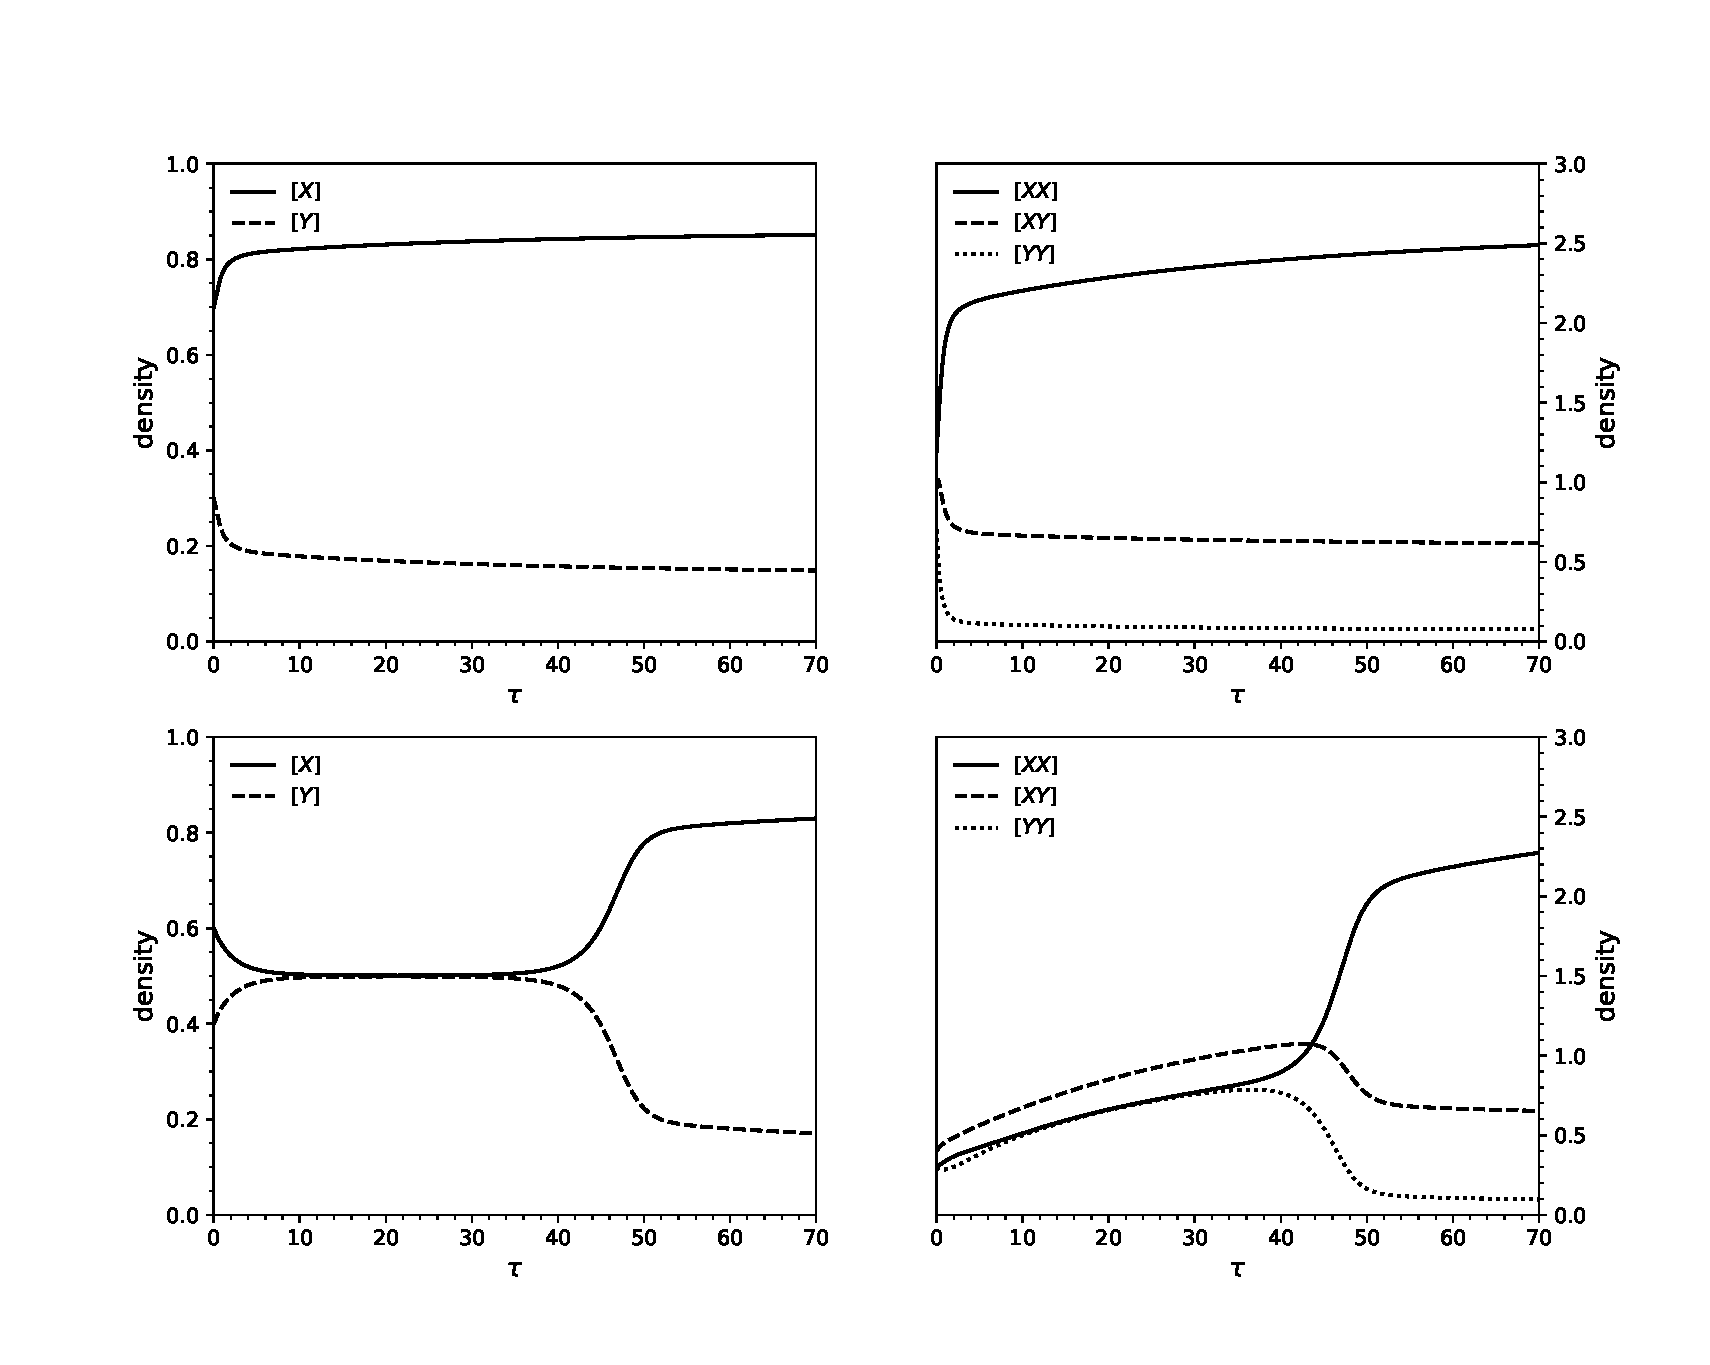
\includegraphics[width = 0.85\textwidth, trim={0 0.5cm 0 2cm},clip=true]{figures/discrete_double_run_1} %trim crops the image on the top such that it fits nicely on the page, trim is activated by option clip=true
		\caption{$\eta = 0.3, \sigma_d = 0.2, \alpha = 0.5, \beta = 0.1$}
		\label{fig:typical_behaviour1}
	\end{subfigure}
	\begin{subfigure}{\textwidth}
		\centering
		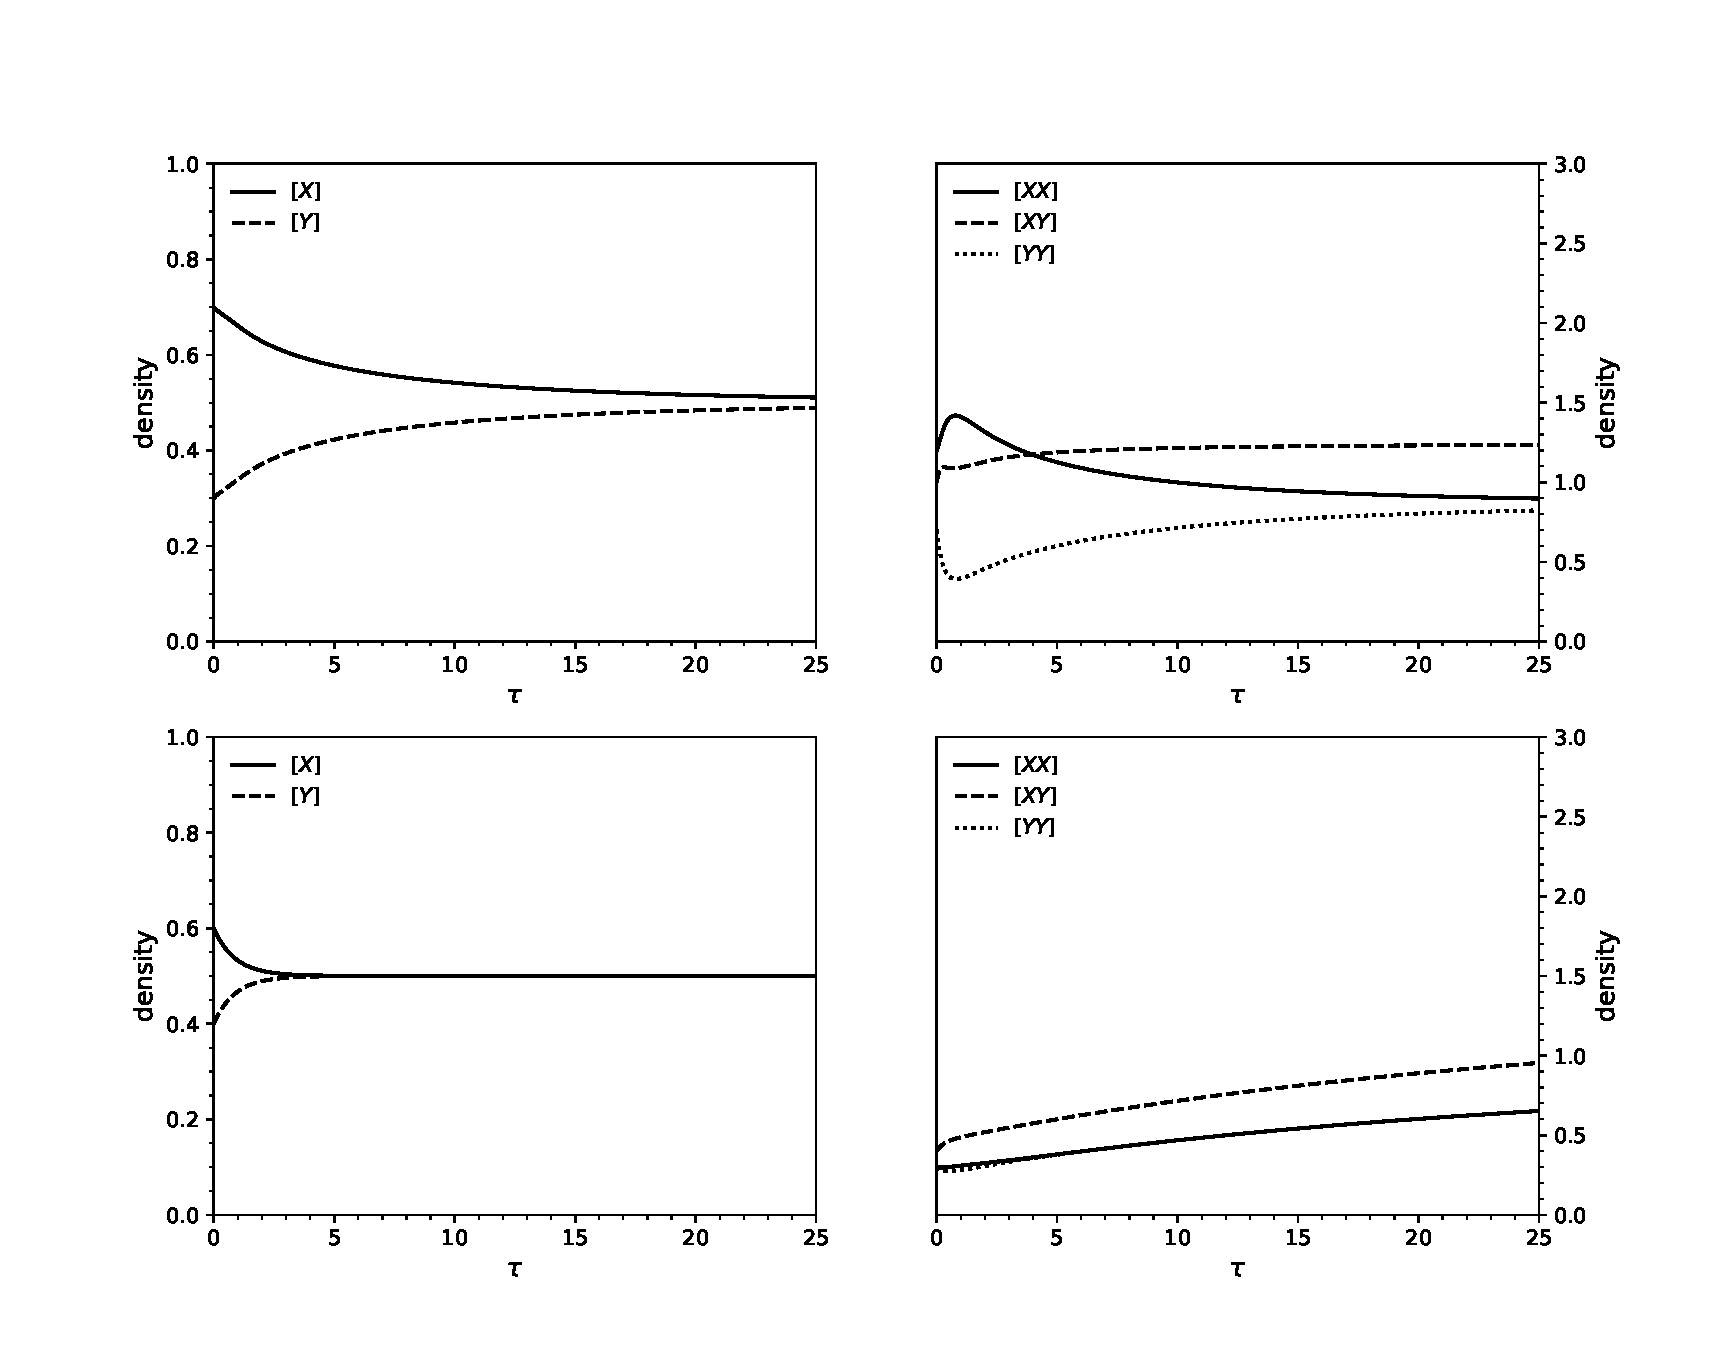
\includegraphics[width = 0.85\textwidth, trim={0 0.5cm 0 1cm},clip=true]{figures/discrete_double_run_2}
		\caption{$\eta = 0.65, \sigma_d = 0.2, \alpha = 0.5, \beta = 0.1$}
		\label{fig:typical_behaviour2}
	\end{subfigure}
	\caption{Behaviour of the two-state adaptive network model for different system parameters and initial conditions. All six figures graph the density of the zeroth moments (left) and the first moments (right) versus the discrete time index $\tau$. In both figure (a) and (b) the initial conditions were taken as $\X=0.7, \Y=0.3, \XX=1.2, \YY=0.7$ $\XY=1.0$ for the upper set of graphs and as $\X=0.6, \Y=0.4, \XX=0.3, \YY=0.3$ $\XY=0.4$ for the lower set. Figures (a) and (b) differ in system parameters $\eta, \sigma_d, \alpha$ and $\beta$.}
%moments1 = [0.7, 0.3, 1.2, 1.0, 0.7]
%moments2 = [0.6, 0.4, 0.3, 0.4, 0.3]
	\label{fig:typical_behaviour}
\end{figure}

In \cref{fig:typical_behaviour2}, the system parameters are chosen such that the system converges to a different stationary solution. This solution is called the \textit{disordered} stationary solution since all states are equally distributed over all nodes. Hence, we have $[\omega] = \frac{1}{M}$ for all $\omega\in\Omega$. In this case, we see that convergence occurs relatively slow if the initial link densities are chosen high, compared to the case where they are lower. Moreover, when the network converges to the disordered solution, it seems that the homogeneous link densities $\XX$ and $\YY$ converge to the same value.

The four different cases in the figure give a good insight into how the system behaves under different conditions. In the next section, we will perform a bifurcation analysis to gain quantitative knowledge of under what conditions the system may and up in what final state.

\section{Bifurcation analysis of the 2-state adaptive network model}

In the previous section, we gained some insight into the behaviour of the two-state adaptive network model. In some cases, the state densities converged to the disordered solution $\X~=~\Y~=~\frac{1}{2}$, while for other system parameters the distributions got very close to the disordered distribution before they converged to their true fixed point.  This behaviour suggests that the disordered solution is either a stable node or a saddle point. In the case of a saddle point, the densities in the unstable manifold might approach the saddle point very slowly before they suddenly shoot away to the final ordered solution. This would also explain the convergence rates. In order to check if this is the case, we will analyse the linear stability in $\X~=~\Y~=~\frac{1}{2}$. 

The two state adaptive network model in \cref{eq:M2system_closure_written_out} can be rewritten as 
\begin{equation}
\bm{\dot{x}} = \bm{f}(\bm{x}),
\end{equation}
for
\begin{equation*}
\bm{x} =
\begin{bmatrix}
\X\\
\Y\\
\XX\\
\YY\\
\XY
\end{bmatrix} 
\hspace{10mm}
\text{and}
\hspace{10mm}
\bm{f}(\bm{x}) = 
\begin{bmatrix}
f_1(\bm{x})\\
f_2(\bm{x})\\
f_3(\bm{x})\\
f_4(\bm{x})\\
f_5(\bm{x})
\end{bmatrix} 
\end{equation*}
where Newton's dot notation is used to indicate the derivative with respect to time $t$. For a solution $\bm{x}^*$ to be a stationary solution (also fixed point, steady state solution or equilibrium solution) we have $\bm{f}(\bm{x}^*)=\bm{0}$ by definition \cite{Strogatz1994}.

%%%%%%%%%%%%%%%%%%%%%%%%%%%%%%%%%%%%%%%%%%%%%%%%%%%%%%%%%%%%%%%%%%%%%%%%%%%%%%%%%%%%%%%%%%%%%

\subsection{Finding fixed points}

In order to obtain expressions for the fixed points of the system, we will be solving $\bm{f}(\bm{x}^*)=\bm{0}$. Therefore, all time derivatives are equated to zero. We start with setting $\frac{d}{dt}\X =0$ or $\frac{d}{dt}\Y=0$, which yields $\X=\Y$ or $\X\Y=\frac{\sigma_d \XY^2}{2\eta}$. Imposing the conservation law $\X+\Y=1$ on the first solution gives $\X=\Y=\frac{1}{2}$. Equating the other time derivatives to zero should give the other coordinates of the fixed point. If we first solve $\frac{d}{dt}\XX= \frac{d}{dt}\YY=0$ we obtain two results, one of which is
\begin{equation}    
\XX=\YY = \frac{\alpha}{8\beta}\frac{ \sigma_d \alpha^2 +4\sigma_d \alpha \beta + 8\eta \beta^2 }{\sigma_d \alpha^2+8\eta \beta^2} = \frac{l}{8}\frac{l^2+4l+8s}{l^2+8s},
\end{equation}
in which we define $l=\frac{\alpha}{\beta}$ as the dimensionless link creation ratio and $s=\frac{\eta}{\sigma_d}$ as the dimensionless noise ratio. 
The other solution is $\eta = 0 \land \left( \sigma_d =0 \lor \XY=0 \right)$. This corresponds to either a network with only link dynamics, implying all node states stay unchanged, or to a network with no flipping noise and no heterogeneous $XY$-links. In the latter case the network is either disconnected or homogeneous such that all nodes are in the same state. Since $\X=\Y=\frac{1}{2}$ and we assume the network is connected this solution can be safely considered as a trivial solution and therefore be omitted. 
Lastly setting $\frac{d}{dt}\XY=0$ gives 
\begin{equation}
\XY = \frac{\alpha}{4\beta} =\frac{l}{4}.
\end{equation}
Combined, the first set of fixed points $\bm{x}^*_1$ is given by 
\begin{equation}
\bm{x}^*_1 = 
\begin{bmatrix}
\frac{1}{2}\\[1ex]
\frac{1}{2}\\[1ex]
\frac{l}{8}\frac{l^2+4l+8s}{l^2+8s}\\[1ex]
\frac{l}{8}\frac{l^2+4l+8s}{l^2+8s}\\[1ex]
\frac{l}{4}
\end{bmatrix},
\end{equation}
corresponding to the disordered stationary solutions. 

We can analyse the stability of the other branch $\X,\Y \neq \frac{1}{2}$ in the same manner. Here we already found $\X\Y=\frac{\sigma_d \XY^2}{2\eta}$. Using the other ODEs, the resulting second set of fixed points $\bm{x}^*_2$ is given as
\begin{equation}
\bm{x}^*_2 = 
\begin{bmatrix}
\frac{1}{2} \pm \frac{1}{2} \sqrt{1-8 \frac{s}{l^2}}\\[1ex]
\frac{1}{2} \mp \frac{1}{2} \sqrt{1-8 \frac{s}{l^2}}\\[1ex]
\frac{s}{l} \left( 1+ \frac{2}{l} \right) \frac{1 \pm \sqrt{1-8\frac{s}{l^2}}}{1 \mp \sqrt{1-8\frac{s}{l^2}}}\\[1ex]
\frac{s}{l} \left( 1+ \frac{2}{l} \right) \frac{1 \mp \sqrt{1-8\frac{s}{l^2}}}{1 \pm \sqrt{1-8\frac{s}{l^2}}}\\[1ex]
\frac{2s}{l}
\end{bmatrix},
\end{equation}
which corresponds to the ordered state solutions. It turns out that the exact density of states $X$ and $Y$ depend on the two system parameters $s$ and $l$ only. Which of the two has the highest density depends on the initial condition; the one with the highest initial density will have the highest stationary state density. 

The fixed points densities are plotted against $s$ for various values of $l$ in the bifurcation diagrams in \cref{fig:bifurcation_zerothM} and \cref{fig:bifurcation_firstM} on the left hand side, whilst they are plotted versus $l$ for various values of $s$ on the right hand side. In \cref{fig:bifurcation_zerothM} we see that for a high noise ratio $s$, the system will converge to a disordered state, while if the noise rate drops below a certain value (depending on $l$), two extra ordered solutions emerge. For low link creation rates $l$ the system also converges to a disordered solution. If $l$ is increased then there is a critical value (depending on $s$) where the same two ordered solutions are formed. From \cref{fig:bifurcation_firstM} we deduce that $l$ determines the density of $XY$-links in the system and that if $l$ is increased, then the overall total number of links increases. On the other hand, higher values of $s$ cause a lower overall link density. If the system converges to an ordered solution, then there are relatively many homogeneous links corresponding to the highest density state, hence, all nodes in the same state will be highly connected. Finally, if the system converges to the ordered state the number of $XY$-links depends linearly on the rate $s$, but if it converges to a disordered state it depends linearly on the rate $l$. 


Finally we note that these fixed points are consistent with the assumption $\alpha\X\Y = \beta\XY$ on both branches, which was made in \cite{Chen2016} to simplify the system in order to allow for analytical evaluation.

\begin{figure}[htp]
	\centering
	\makebox[\textwidth][c]{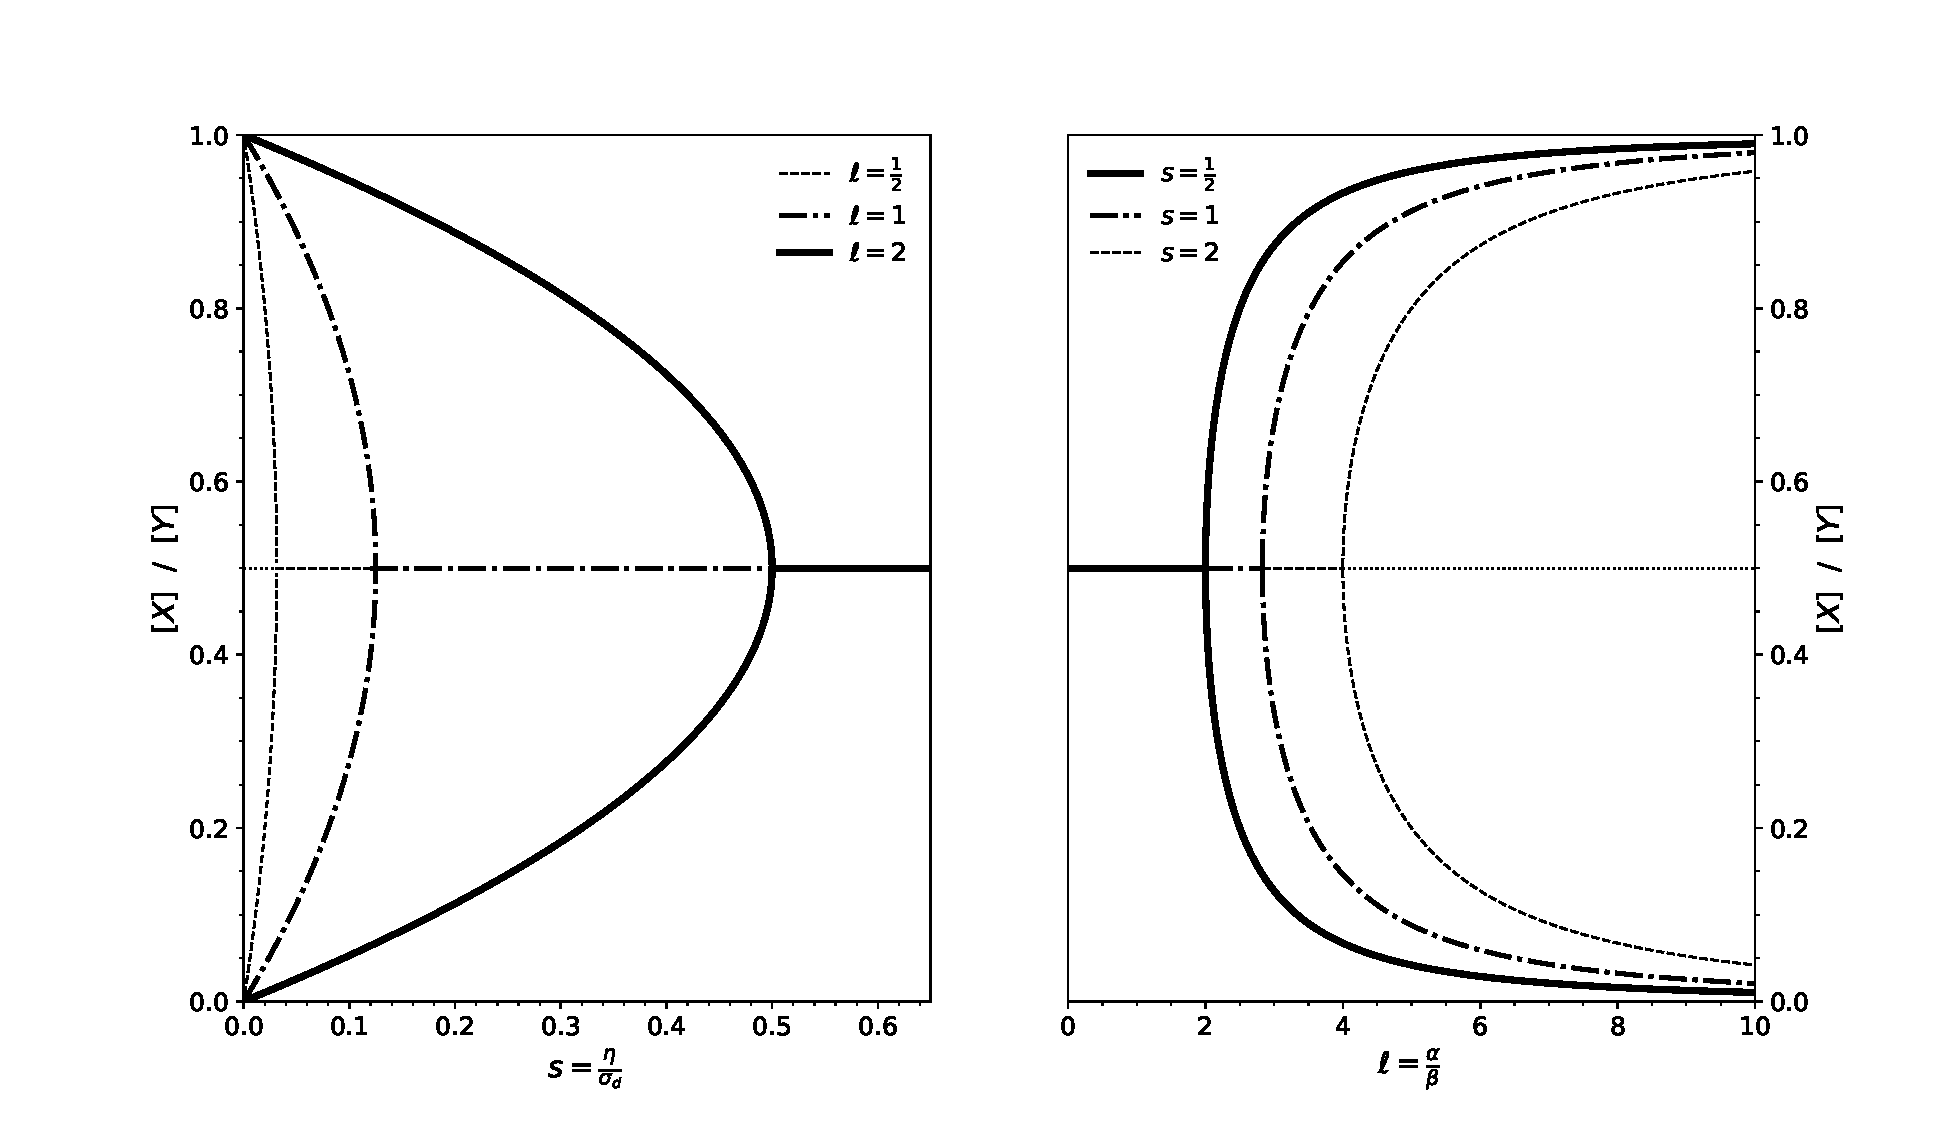
\includegraphics[width = 1.1\textwidth]{figures/bifurcation_zeroth}}
	\caption{Bifurcation diagrams of the two state adaptive network model. The ordered and disordered stationary solutions of state densities $\X, \Y$ for various values of the link creation parameter $l$ as function of the noise ratio $s$ (left) and for various values of $s$ as function of $l$ (right). Both stable and unstable solutions are plotted. The bifurcation is a supercritical pitchfork bifurcation.}
	\label{fig:bifurcation_zerothM}
\end{figure}
\begin{figure}[htp]
	\centering
	\begin{subfigure}{\textwidth}
		\centering
		\makebox[\textwidth][c]{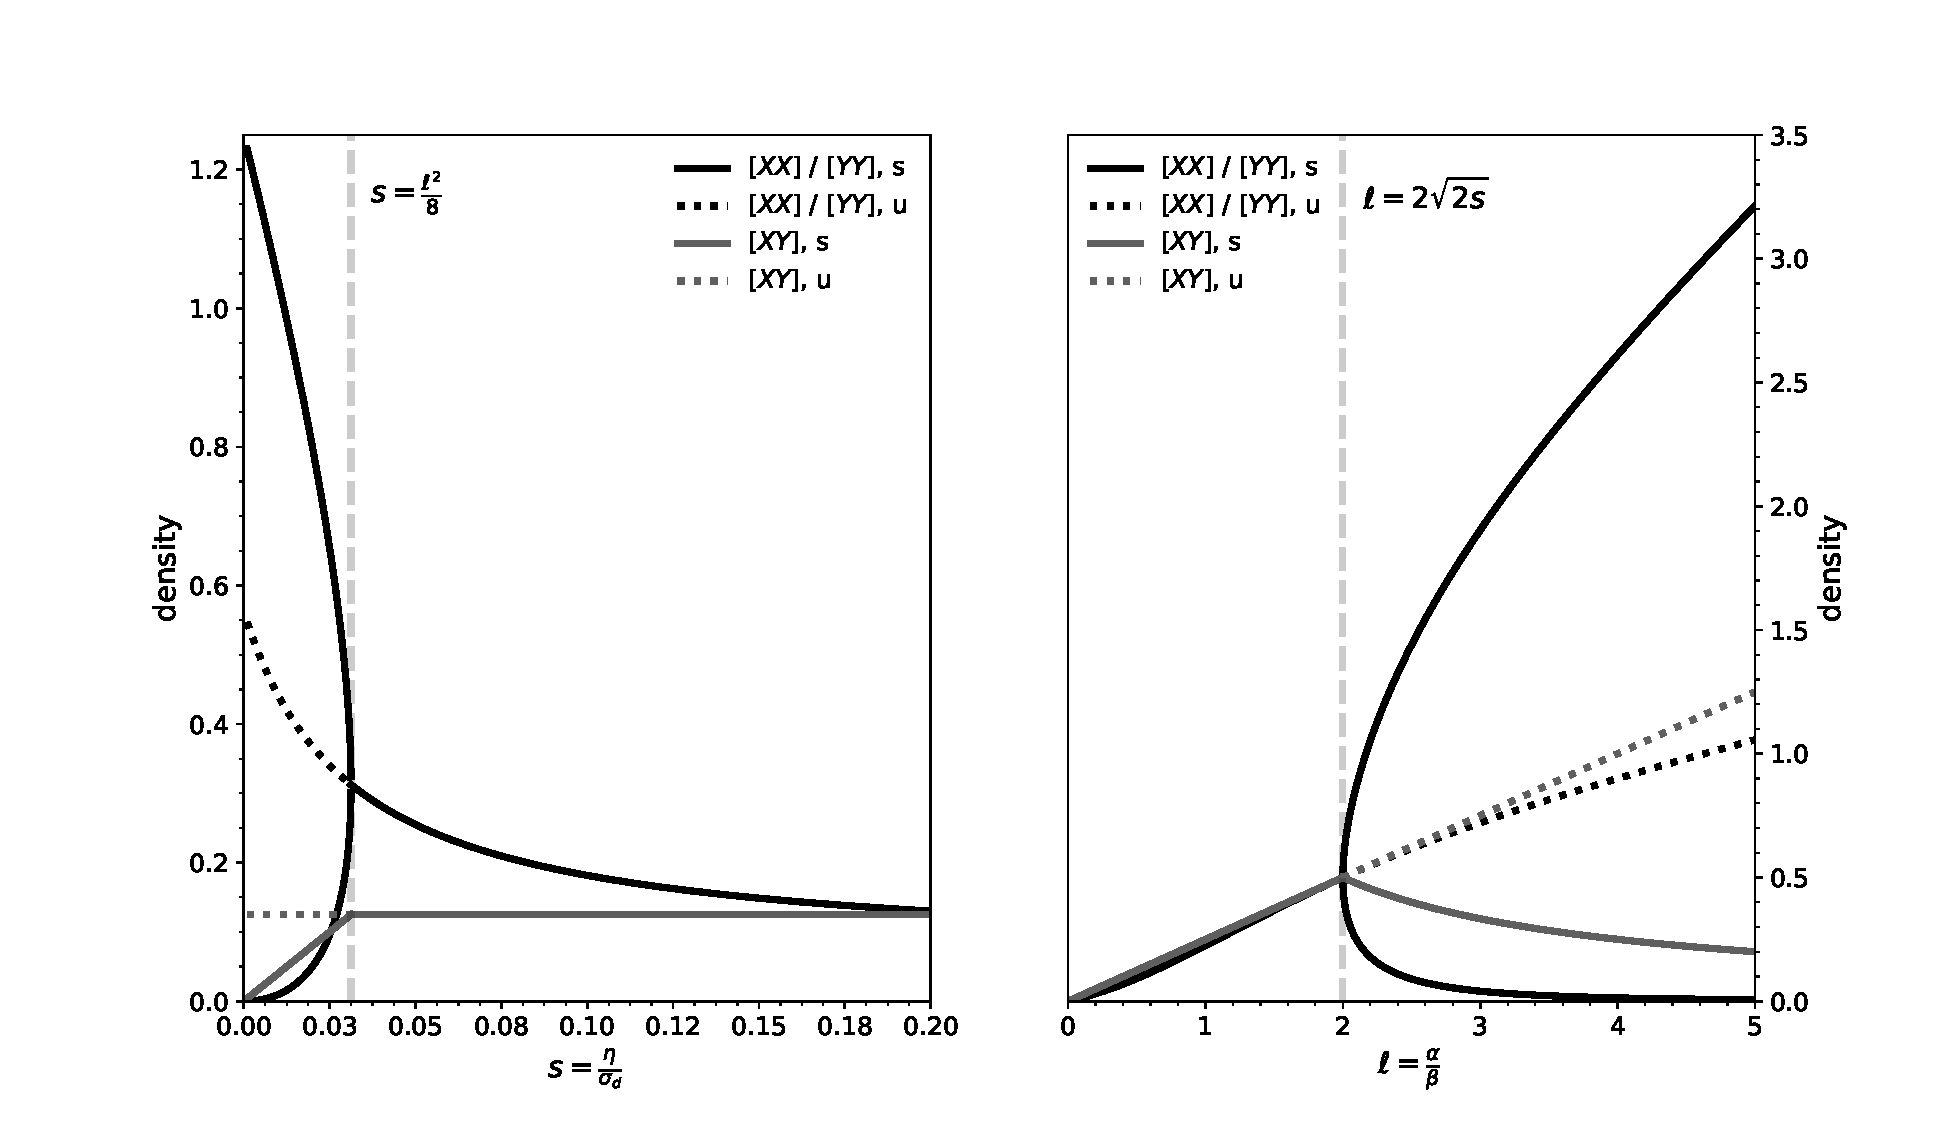
\includegraphics[width = 1.1\textwidth, trim={0 0cm 0 0cm},clip=true]{figures/bifurcation_first_s_05_l_05_BW}}% %trim crops the image on the top such that it fits nicely on the page, trim is activated by option clip=true
		\caption{\qquad\qquad $l=\frac{1}{2}$ \hspace{4.8cm} $s=\frac{1}{2}$ \qquad\qquad\quad}
		\label{}
	\end{subfigure}
	\begin{subfigure}{\textwidth}
		\centering
		\makebox[\textwidth][c]{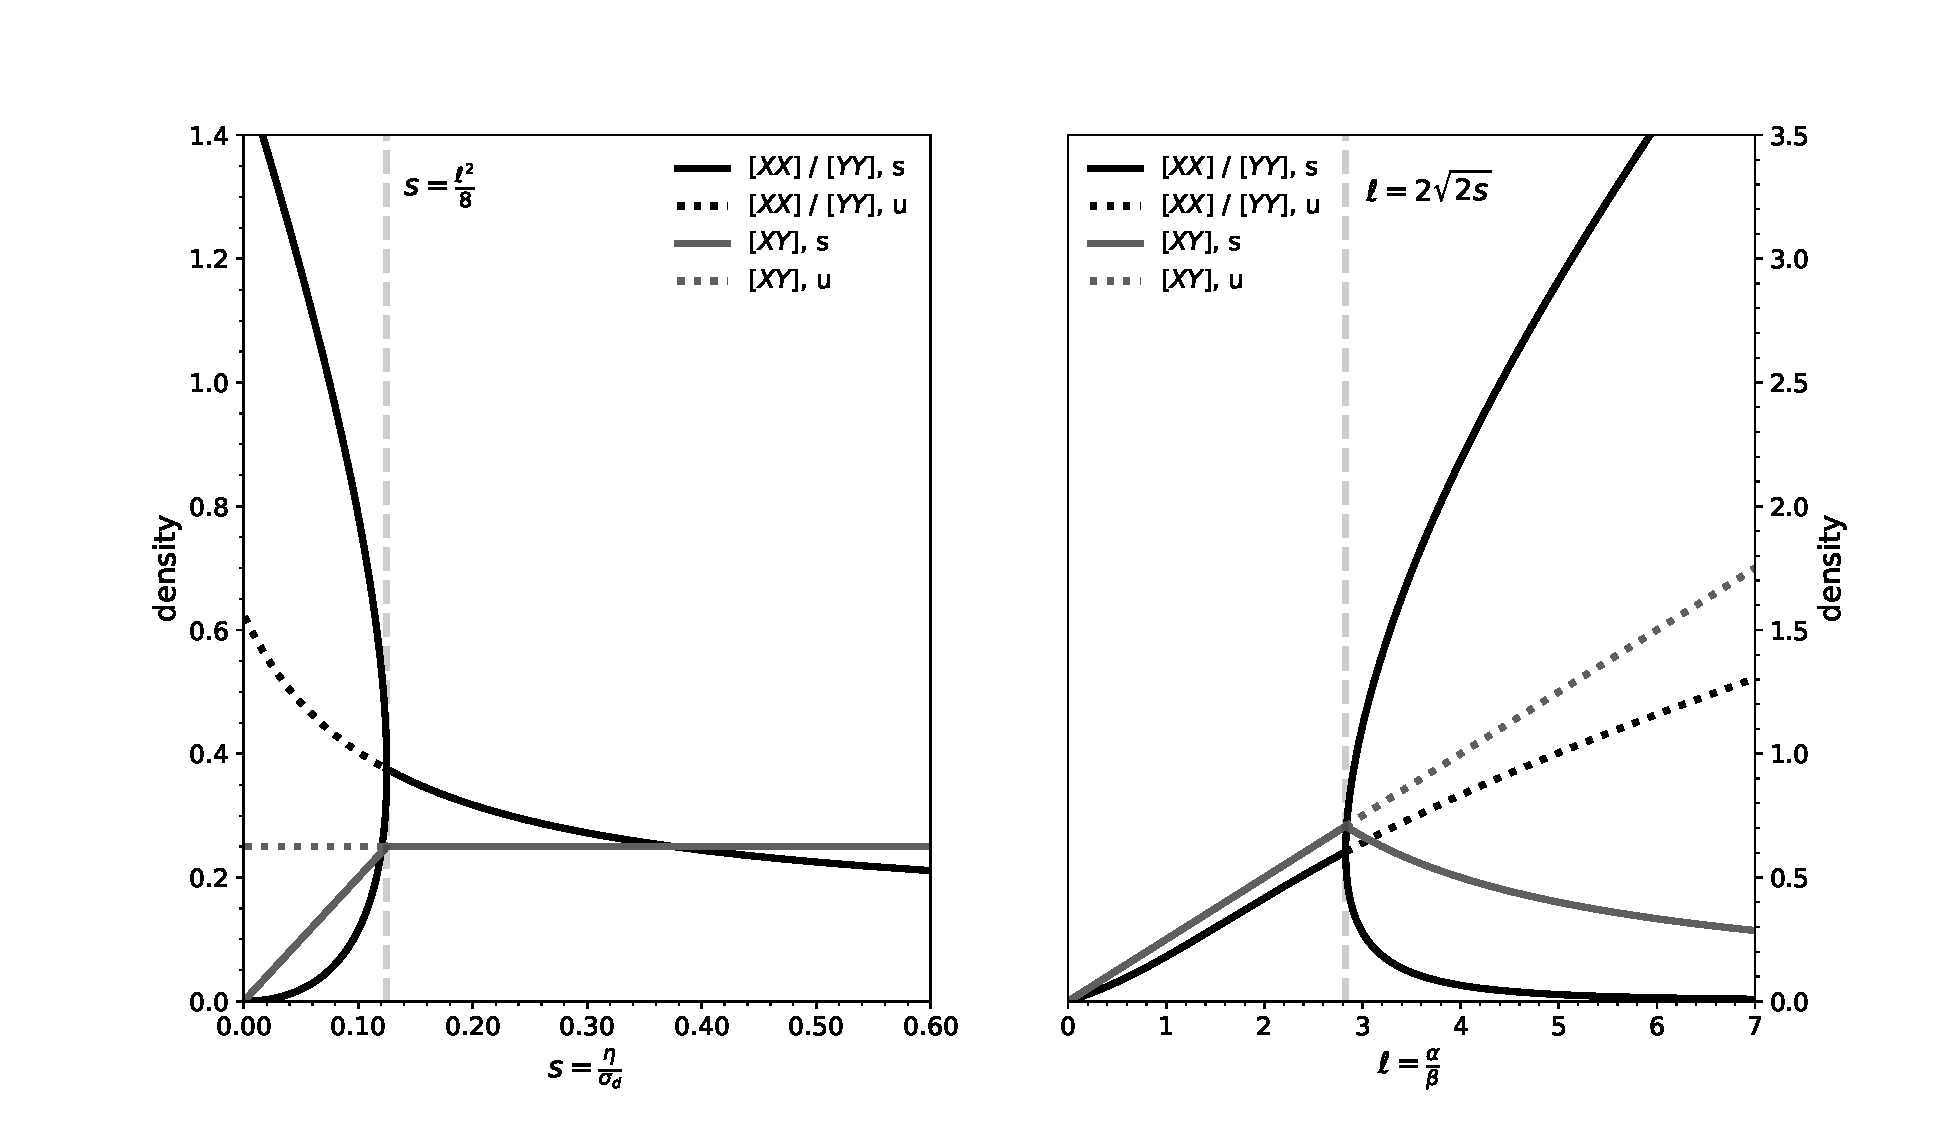
\includegraphics[width = 1.1\textwidth, trim={0 0cm 0 0cm},clip=true]{figures/bifurcation_first_s_1_l_1_BW}}
		\caption{\qquad\qquad $l=1$ \hspace{4.8cm} $s=1$ \qquad\qquad\quad}
		\label{}
	\end{subfigure}
	\caption{(continues on next page)}
\end{figure}
\clearpage
\begin{figure}[htp]
	\ContinuedFloat
	\begin{subfigure}{\textwidth}
		\centering
		\makebox[\textwidth][c]{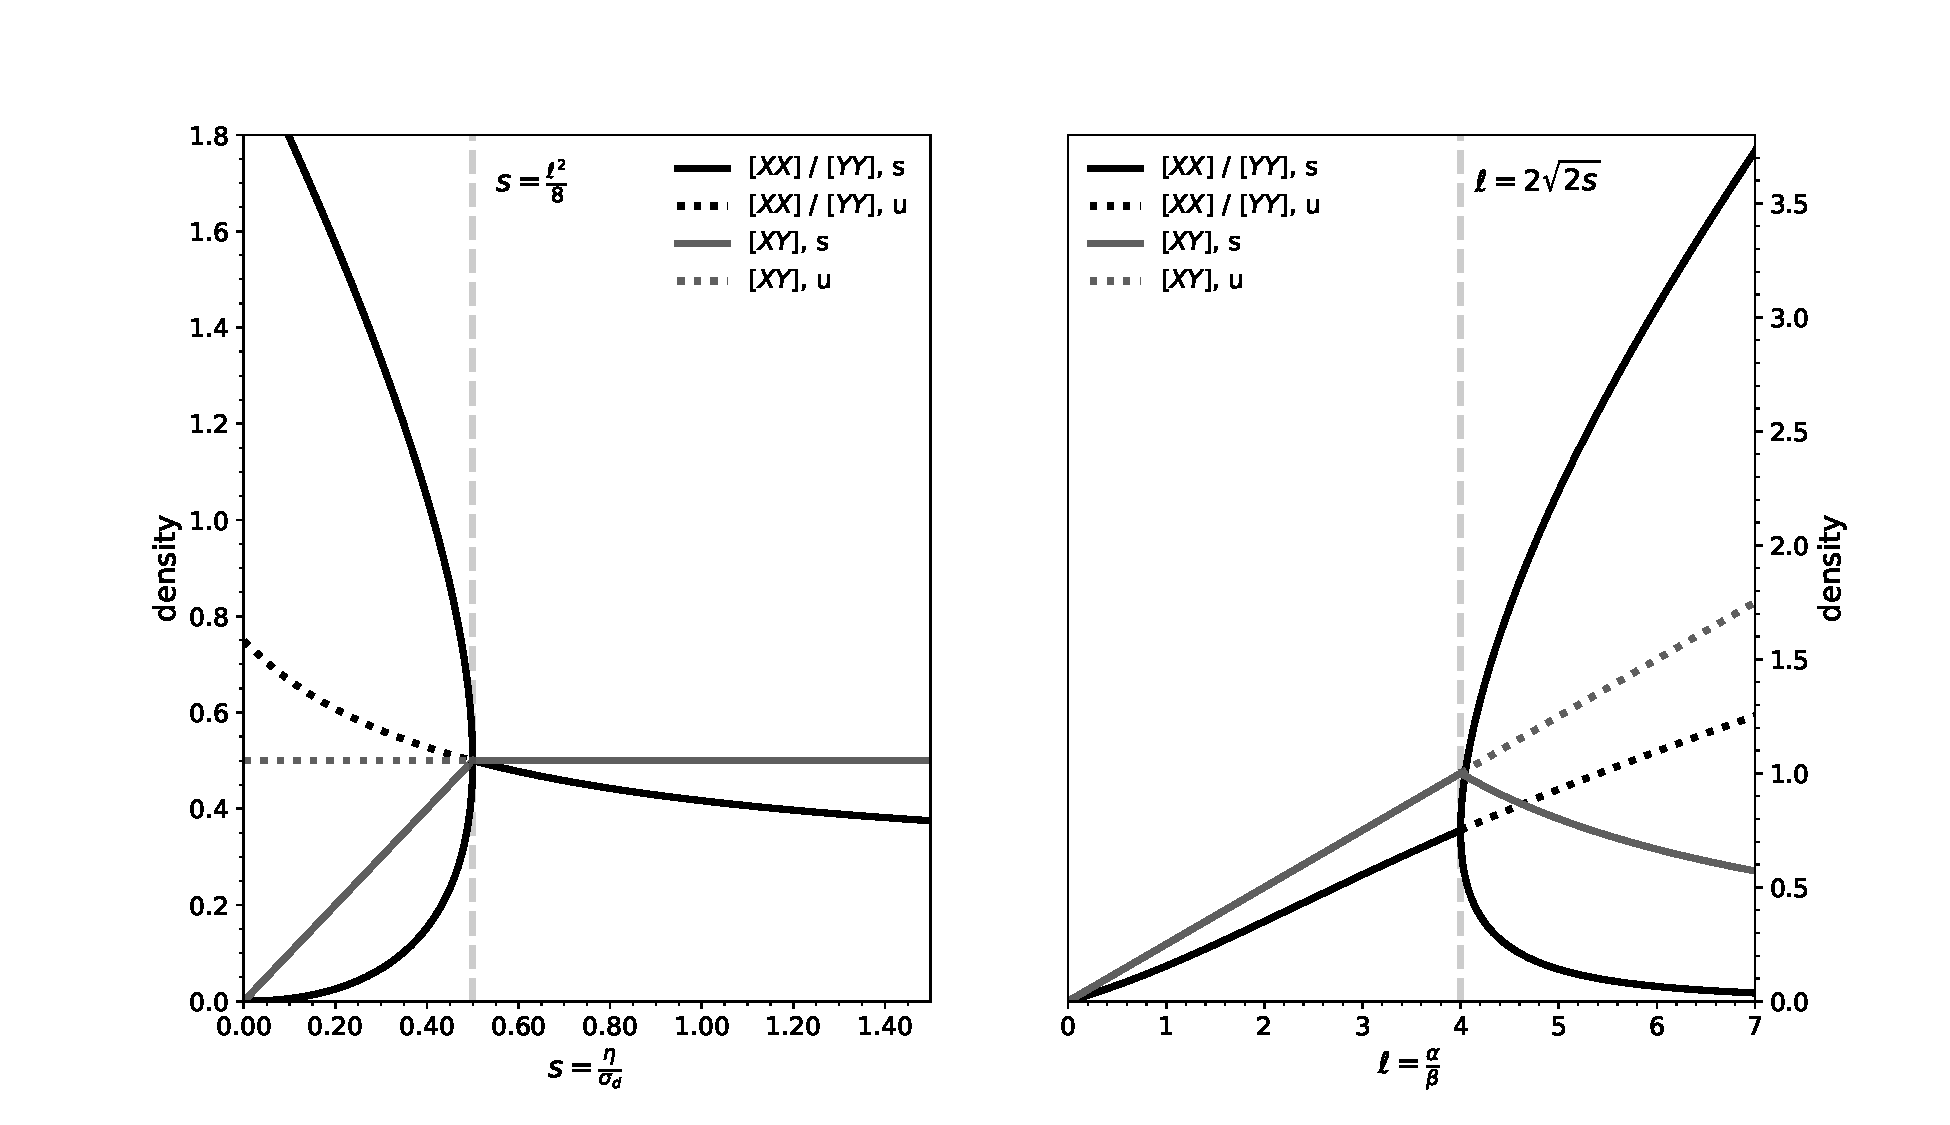
\includegraphics[width = 1.1\textwidth, trim={0 0cm 0 0cm},clip=true]{figures/bifurcation_first_s_2_l_2_BW}}
		\caption{\qquad\qquad $l=2$ \hspace{4.8cm} $s=2$ \qquad\qquad\quad}
		\label{}
	\end{subfigure}
	\caption{Bifurcation diagrams of the two state adaptive network model. (left) The stationary solutions of link densities $\XX, \YY, \XY$ for various values of the link creation parameter $l$ as function of the noise ratio $s$. The stable disordered stationary solutions are on the right hand side of the line $s=\frac{l^2}{8}$, while the unstable disordered solutions are on the left hand side plotted with a dotted line. The bold curves on the left hand side indicate the ordered stationary solutions. (right) The stationary solutions of link densities $\XX, \YY, \XY$ for various values of $s$ as function of $l$. The stable disordered stationary solutions are on the left hand side from the line $l=2\sqrt{2s}$, while the unstable disordered solutions are on the right hand side plotted with a dotted line. The bold curves on the right hand side indicate ordered stationary solutions. Note that the axis scales differ. }
	\label{fig:bifurcation_firstM}
\end{figure}

\subsection{Linearisation}
For further stability analysis, we will proceed with a linearisation of the system of ODEs around its fixed points $\bm{x}^*$. This can be done as follows
\begin{equation}
\begin{aligned}
\bm{f}(\bm{x}^* + \Delta \bm{x}) 
&= \bm{f}( \bm{x}^* ) + J\rvert_{ \bm{x}^* }  \Delta \bm{x}  + \mathcal{O}(\Vert \Delta \bm{x} \Vert^2_2)\\
&\approx J\rvert_{ \bm{x}^* }  \Delta \bm{x},
\end{aligned}
\end{equation} 
in which the Jacobian matrix $J$ is defined component-wise by $J_{i,j} = \frac{\partial f_i}{\partial x_j}$ with $x_j$ an element of $\bm{x}$.
Now in order to evaluate the stability of the found fixed points, we will need the theorem of Lyapunov, which enables us to find the stability by evaluation of the eigenvalues of the Jacobian matrix. The proof is not written out here, since it can be found in various books on basic differential equation or bifurcation theory, for example \cite{Boyce2010, Braun1993}.

\begin{theorem}[Lyapunov]
	Let $f: \mathbb{R}^n \to \mathbb{R}^n$ be an element of $C^1$ and $\bm{x}^*$ be a fixed point of $\bm{\dot{x}} = \bm{f}(\bm{x})$. Let $\bm{\dot{x}} = J\rvert_{ \bm{x}^* }  \bm{x}$ be the linearization of $f$ with $J$ the Jacobian matrix with eigenvalues $\lambda_1,..,\lambda_n$. $\bm{x}^*$ is
	\begin{enumerate}
		\item asymptotically stable if $\Re \lambda_i < 0$ for all $i \in \{1,...,n\}$,
		\item unstable if $\Re \lambda_i > 0$ for some $i \in \{1,...,n\}$
	\end{enumerate}
\end{theorem}
Note that the theorem does not say anything if $\Re \lambda_i = 0$ for some $i \in \{1,...,n\}$. Hence, further analysis is necessary in that case. This theorem is applicable since $\bm{f}$ is continuous in time $t$. Using Maple 2018 the Jacobian matrix is evaluated in the first set of fixed points $\bm{x}^*_1$. The resulting five eigenvalues can be written as
\begin{subequations}
	\label{eq:eigenvalues}
	\begin{alignat}{3}
	\lambda_1 &= 0& \\
	\lambda_2 &= 
	\frac{\phantom{-} \sigma_d \alpha^2 - 8\eta \beta^2}{4\beta^2} 
	&& = \phantom{-} \frac{1}{4}\sigma_d l^2 -2\eta\\  %phantom is used to align the fractions. it replaces the exact space the minus sign takes with white space
	\lambda_3 &= 
	\frac{- \sigma_d \alpha^2 - 8\eta \beta^2}{4\beta^2} 
	&& = -\frac{1}{4}\sigma_d l^2 -2\eta\\
	\lambda_4 &= \frac{\phantom{-}\sqrt{b^2-4ac}-b}{2a} & \\
	\lambda_5 &= \frac{-\sqrt{b^2-4ac}-b}{2a},  &
	\end{alignat}
\end{subequations}
where the latter two eigenvalues are written in terms of a certain $a, b, c \in \mathbb{R}_{>0}$, which are quite elaborate expressions in terms of parameters $\eta, \sigma_d, \alpha$ and $\beta$.  

According to the theorem, each eigenvalue with negative real part corresponds to an asymptotically stable manifold of the fixed point $\bm{x}^*_1$ in the phase plane, whilst each eigenvalue with positive real part will have an eigenvector corresponding to an unstable manifold. Before evaluating these eigenvalues, note that $\lambda_1$ is a zero eigenvalue, which emerges because the conservation law $\X+\Y=1$ is imposed on the system. In fact, this directly implies that there only exist valid solutions to the system of ODEs in a four-dimensional subspace of the five-dimensional $\left( \X, \Y, \XX, \YY, \XY \right)$ space. These statements are formalized in the following theorem. 

\begin{theorem}
	\label{th:conservation_implies_zero_eigenvalue}
	If a conservation law is imposed on a system of first order ODEs, then the corresponding Jacobian matrix $J$ has at least one eigenvalue zero.
\end{theorem}
\begin{proof}
	Let $\dot{\bm{x}} = \bm{f}(\bm{x})$ be a system of first order ODEs in which $\bm{x} = [x_1, x_2, ..., x_n]^T$ and $\bm{f(x)} = [f_1(\bm{x}), f_2(\bm{x}), ..., f_n(\bm{x})]^T$. Furthermore suppose there is a conservation law, which means that a certain linear combination of time derivatives equals zero. This law enables us to express one derivative in terms of the other derivatives. Assume without loss of generality  $\dot{x_1}=h(\dot{x}_2,...,\dot{x}_n)$, with $h$ a linear function. Using the system of equations we then find $f_1(\bm{x}) = \dot{x_1}=h(\dot{x}_2,...,\dot{x}_n) = h(f_2(\bm{x}), ..., f_n(\bm{x}))$.
	
	The Jacobian matrix $J$ is defined as
	\begin{equation*}
	\begin{aligned}
	J = \frac{\partial (f_1,...,f_n)}{\partial (x_1,...,x_n)}
	&=  
	\begin{bmatrix}
	\frac{\partial f_1}{\partial x_1} &
	\frac{\partial f_1}{\partial x_2} &
	\dots & 
	\frac{\partial f_1}{\partial x_n} \\[1ex] % <-- 1ex more space between    rows of matrix
	\frac{\partial f_2}{\partial x_1} &
	\frac{\partial f_2}{\partial x_2} &
	\dots & 
	\frac{\partial f_2}{\partial x_n} \\[1ex] % <-- 1ex more space between    rows of matrix
	\vdots & 
	\vdots &
	\ddots & 
	\vdots \\[1ex]
	\frac{\partial f_n}{\partial x_1} &
	\frac{\partial f_n}{\partial x_2} &
	\dots & 
	\frac{\partial f_n}{\partial x_n}
	\end{bmatrix}\\[1ex]
	&=  
	\begin{bmatrix}
	\frac{\partial h(f_2(\bm{x}), ..., f_n(\bm{x}))}{\partial x_1} &
	\frac{\partial h(f_2(\bm{x}), ..., f_n(\bm{x}))}{\partial x_2} &
	\dots & 
	\frac{\partial h(f_2(\bm{x}), ..., f_n(\bm{x}))}{\partial x_n} \\[1ex] % <-- 1ex more space between    rows of matrix
	\frac{\partial f_2}{\partial x_1} &
	\frac{\partial f_2}{\partial x_2} &
	\dots & 
	\frac{\partial f_2}{\partial x_n} \\[1ex] % <-- 1ex more space between    rows of matrix
	\vdots & 
	\vdots &
	\ddots & 
	\vdots \\[1ex]
	\frac{\partial f_n}{\partial x_1} &
	\frac{\partial f_n}{\partial x_2} &
	\dots & 
	\frac{\partial f_n}{\partial x_n}
	\end{bmatrix}\\[1ex]
	&=  
	\begin{bmatrix}
	h\left( \frac{\partial f_2}{x_1},...,\frac{\partial f_n}{x_1} \right) &
	h\left( \frac{\partial f_2}{x_2},...,\frac{\partial f_n}{x_2} \right) &
	\dots & 
	h\left( \frac{\partial f_2}{x_n},...,\frac{\partial f_n}{x_n} \right) \\[1ex] % <-- 1ex more space between    rows of matrix
	\frac{\partial f_2}{\partial x_1} &
	\frac{\partial f_2}{\partial x_2} &
	\dots & 
	\frac{\partial f_2}{\partial x_n} \\[1ex] % <-- 1ex more space between    rows of matrix
	\vdots & 
	\vdots &
	\ddots & 
	\vdots \\[1ex]
	\frac{\partial f_n}{\partial x_1} &
	\frac{\partial f_n}{\partial x_2} &
	\dots & 
	\frac{\partial f_n}{\partial x_n}
	\end{bmatrix}.
	\end{aligned}
	\end{equation*}
	Since $h$ is a linear function, it is possible to find a matrix $A$ which defines row operations such that $A J $ has a row containing only zeros. This implies $\det(AJ) = 0 = \det(AJ-\lambda I)$ for $\lambda=0$. Therefore $AJ$ has an eigenvalue $\lambda=0$. It follows directly that the Jacobian matrix $J$ also has an eigenvalue $\lambda=0$, since row operations leave the eigenvalues unchanged.
\end{proof}

Because the Jacobian matrix has one row which is linearly dependent on the other rows, $\text{rank}( J) \leq n-1$. This means that the solutions to the system are all found on a subspace of maximum dimension $n-1$ of the phase space. This also means that the system can be reduced to an identical four-dimensional system, in which the zero eigenvalue disappears. Therefore $\lambda_1=0$ does not influence the stability. 

Looking at the other eigenvalues, we see that $\lambda_2$ and $\lambda_3$ differ by a minus sign. Demanding $\lambda_2 < 0$ gives 
\begin{equation}
l^2<8s,
\end{equation}
as a condition for asymptotic stability of $\bm{x}_1^*$. Furthermore, since $\eta, \sigma_d, \alpha, \beta > 0$ we have $\lambda_3 < 0$. The last two eigenvalues $\lambda_4$ and $\lambda_5$ also differ by a minus sign. Using Maple, it was verified that $0 < 4ac < b^2$, which implies $\sqrt{b^2-4ac}  < b$. Since $2a > 0$ we have $\lambda_4 < 0$. Also using the fact that $a, b, c > 0$ it can be concluded that $ \lambda_5 < 0$.

Altogether, $\lambda_1$ does not influence the stability, $\lambda_2$ demands $l^2 < 8s$ for a stable manifold in the phase plane and $\lambda_3, \lambda_4, \lambda_5 < 0$ create stable manifolds in all cases. This makes $\bm{x}^*_1$ a stable node in phase space for $l^2 < 8s$ and a 1-saddle point if this condition is not met. This means that the curve $l^2 = 8s$, or $l = 2\sqrt{2s}$, represents supercritical pitchfork bifurcations of the two-state adaptive network model\footnote{Since we go from one unstable and two stable fixed points to one stable fixed point this is a supercritical pitchfork and not a saddle-node bifurcation \cite{Kuznetsov2004}.}. 

For determining the stability of the second set of fixed points $\bm{x}^*_2$ the same procedure could be followed. However, it turns out that apart from one zero eigenvalue, four over 25-degree polynomials in the four system parameters $\alpha, \beta, \eta, \sigma_d$ are found. Unfortunately, there is no way to simplify them, so for a stability condition a different approach is needed. With the MATLAB-package MatCont, which can be used for numerical bifurcation analysis of dynamical systems \cite{Dhooge2008}, one can check and search for additional bifurcations in a system. After a normal time integration, where the software finds the fixed point $\bm{x}_2^*$, it analyses the behaviour of the eigenvalues numerically to find these special points. We find that the system is only to end up in the disordered solution if $l^2>8s$, which is the exact opposite requirement compared to the ordered solution. Derivatives up to the third order were computed analytically using the Symbolic Math Toolbox.

As a whole, we find that the pitchfork bifurcations are found on $l^2=8s$, moreover, these are the only bifurcations in the system. For $l^2 < 8s$ the disordered solution $\bm{x}_1^*$, in which all states in $\Omega$ are equally distributed over all nodes, is the only stable node. Hence all systems will converge to that same state, irrespective of the initial condition. For $l^2 > 8s$ the ordered solution $\bm{x}_2^*$ is a stable node and the disordered solution $\bm{x}_1^*$ a 1-saddle point. All systems will therefore eventually converge to $\bm{x}_2^*$, given that the initial condition of the system is not on the stable manifold of $\bm{x}_1^*$

In addition, MatCont was used to confirm all analytic results in this section. For various combinations of $s$ and $l$ the final state distribution at time $t_f=1000$ was plotted either as cross if it converged to an ordered state or as a square if it ended up in a disordered state in \cref{fig:phase_diag_M2}. The curve $s=2\sqrt{2s}$ indicates the supercritical pitchfork bifurcation. The numerical solutions are perfectly in line with the analytic derivation. Hence, irrespective of what biological, physical or social system the adaptive network is applied to, we know the outcome once we know the initial condition and the values of the system parameters $s=\frac{\eta}{\sigma_d}$ and $l=\frac{\alpha}{\beta}$. 

\begin{figure}[htp]
	\centering
	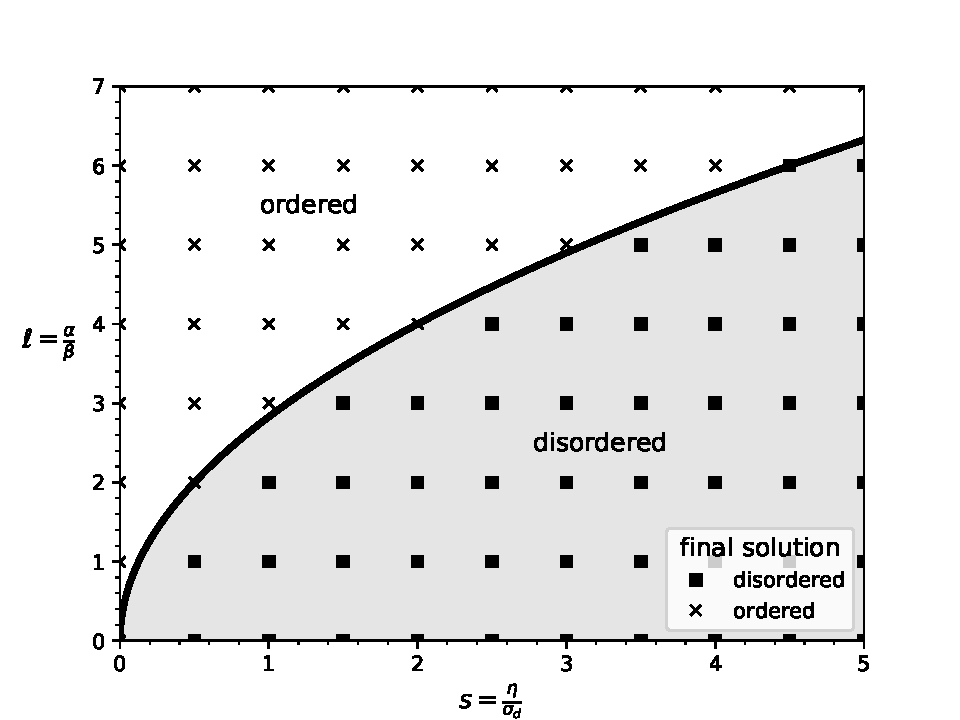
\includegraphics[width=0.7\linewidth, trim={0 0 0 1cm},clip=true]{figures/phase_diag_M2_sims}
	\caption{Phase diagram of a two-state adaptive network model as described by \cref{eq:M2system_closure_written_out}. The diagram displays the stable stationary state solution as a function of the dimensionless noise ratio $s=\frac{\eta}{\sigma_d}$ and the dimensionless link creation ratio $l=\frac{\alpha}{\beta}$. For $l<2\sqrt{2s}$, the disordered solution is stable, whilst for $l>2\sqrt{2s}$ the system will converge to the ordered solution. At the curve $l=2\sqrt{2s}$ there is a supercritical pitchfork bifurcation. Final distributions in numerical solutions for various $s$ and $l$ are indicated by the squares and crosses for the disordered and the ordered solution respectively. }
	\label{fig:phase_diag_M2}
\end{figure}

